\documentclass{standalone}

\usepackage{tikz}
\usepackage{ctex}

\begin{document}
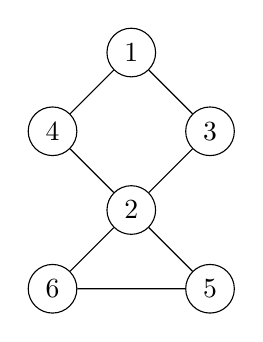
\begin{tikzpicture}

\begin{scope}[every node/.style=draw,circle]
    \node (A) at (0,2) {$1$};
    \node (B) at (0,0) {$2$};
    \node (C) at (1,1) {$3$};
    \node (D) at (-1,1) {$4$};
    \node (E) at (1,-1) {$5$};
    \node (F) at (-1,-1) {$6$};
\end{scope}

\draw
    (A) -- (C)
    (A) -- (D)
    (C) -- (B)
    (D) -- (B)
    (B) -- (E)
    (B) -- (F)
    (E) -- (F);

\end{tikzpicture}
\end{document}
